\documentclass[11pt]{article}

\usepackage[utf8]{inputenc}
\usepackage{mathtools}
\usepackage{amsmath}
\usepackage{amsfonts}
\usepackage{enumerate}

% For proper referencing in article
\usepackage{hyperref}
\usepackage{url}

% For figures and graphics'n stuff
\usepackage{graphicx}
\usepackage{caption}
\usepackage{subcaption}
% \usepackage{tabularx}
\usepackage{float}

% For proper appendices
\usepackage[toc,page]{appendix}

% Algorithm packages
\usepackage{algorithm}
\usepackage{algorithmicx}
\usepackage{algpseudocode}

% For bold math symbols
\usepackage{bm}
\usepackage{xcolor}

% For customized hlines in tables
\usepackage{ctable}

% For having latex symbols in section titles
\usepackage{epstopdf}

% For proper citations
% \usepackage[round, authoryear]{natbib}
\usepackage[numbers]{natbib} 

% For fixing large table height
\usepackage{a4wide}

% Remembrance and checking
\newcommand{\husk}[1]{\color{red} #1 \color{black}}
\newcommand{\sjekk}[1]{\color{violet} #1 \color{black}}

\DeclareMathOperator{\sign}{sign}
\DeclareMathOperator*{\argmin}{argmin}
\DeclareMathOperator*{\CO}{\mathcal{C}}


% \title{FYS-STK4155: Project 2}
\title{Exploring the hyperspace of Machine Learning parameters}
\author{Eirik Ramsli Hauge, Joakim Kalsnes, Hans Mathias Mamen Vege}
\date{\today}

\begin{document}
\maketitle

\begin{abstract}
NaN
\end{abstract}

% \tableofcontents

%%%%%%%%%%%%%%%%%%%%%%%%%%%%%%%%
\section{Introduction}


%%%%%%%%%%%%%%%%%%%%%%%%%%%%%%%%
% Theory introduction goes here

\section{Theory}
\subsection{The Ising Model} \label{sec:ising-model}
The Ising model is a way of modeling phase transitions at finite temperatures of magnetic systems. When modeling, we set up a chain or a lattice of particles and allow them to have either spin up or spin down. From this, one can sample energy and magnetization, and measure several quantities such as the heat capacity or magnetic susceptibility. Our focus will be on predicting the energy coupling constant for a 1D lattice, and the phase of a 2D-lattice.

Periodic boundary conditions is given in both cases, such that $j=N=0$, where $j$ is the lattice site and $N$ is the lattice size.

\subsubsection{1-dimensional Ising model} \label{sec:1d-ising-model}
Energy for a 1 dimensional Ising model is given as
\begin{align}
    E = - J\sum^N_{j=1} s_j s_{j+1}
    \label{eq:1d-ising-energy}
\end{align}
where the $N$ is the number of particles(or lattice size) and s$_j=\pm1$ is the j'th spin. Our goal will be to predict $J$, but in order to do so, we must recast the problem as a linear regression problem.

We begin by labeling each site as coupled with $J$.
\begin{align}
    E_\mathrm{model}[\bm{s}^i] = -\sum^N_{j=1} \sum^N_{k=1} J_{j,k} s^i_j s^i_k,
\end{align}
where $i$ is the index over lattice configurations. The coupling strength $J_{j,k}$  can now be cast as a matrix, and we end up with
\begin{align}
    E_\mathrm{model}^i \equiv \bm{X}^i \cdot \bm{J},
    \label{eq:1d-ising-linreg}
\end{align}
where $\bm{X}^i$ is the design matrix consisting of all two-body interactions $\{s^i_j s^i_k\}^N_{j,k=1}$, and $\bm{J}$ the weight matrix we wish to find later using machine learning techniques.

\subsubsection{2-dimensional Ising model} \label{sec:2d-ising-model}
The 2D Ising model has its energy stated as,
\begin{align}
    E = - J\sum^N_{<kl>} s_k s_l,
    \label{eq:2d-ising-energy}
\end{align}
where $<kl>$ indicates a sum over the nearest neighbors. That is, written out,
\begin{align}
    E = - J\sum^N_{i,j} 2 s_{i,j} (s_{i+1,j} + s_{i-1,j} + s_{i,j+1} + s_{i,j-1}),
    \label{eq:2d-ising-energy-shortened}
\end{align}
where we have used the symmetry that $s_{i,j} s_{i+1,j}=s_{i+1,j} s_{i,j}$. $J$ is, as in the 1D model, a coupling constant, but will not be our main focus when studying the 2D Ising model. This time, we will focus on its property of exhibiting phase transitions. Below a critical temperature of $T_C \approx 2.269$ found analytically by \citep{onsager1944crystal}, the lattice will exhibit an ordered state, one in which the spins is \textit{locked} or \textit{frozen} into place. Above $T_C$ the lattice exhibit a disordered phase, as the spins will be fluctuating randomly.

We will investigate the classification of states below $T<2.0$ and $T>2.5$. The phase for states between we will dub as being in a \textit{critical phase}.

\subsection{Logistic regression}
\documentclass[12pt]{article}

\usepackage{amsmath}
\DeclareMathOperator*{\argmin}{argmin}
\usepackage{bm}
\usepackage{xcolor}

\newcommand{\husk}[1]{\color{red} #1 \color{black}}
\newcommand{\sjekk}[1]{\color{violet} #1 \color{black}}

\begin{document}
\section{Theory}
In project 1 we used linear regression to predict a continuous output from a set of inputs (\husk{reference project1}). We used ordinary least squares regression (OLS), Ridge regression and Lasso regression, where the two latter impose a penalty to the OLS. In this project we will reuse the ideas and code of project 1, but we will also use neural networks to predict continuous variables. In addition we study situations where the outcome is discrete rather than continuous. This is a classification problem, and we will use logistic regression to model the probabilities of the classes.\\

\subsection{Logistic regression}
Just like a linear regression model, a logistic regression model computes a weighted sum of the predictor variables, written in matrix notation as $\bm{X}^T\beta$. However, the logistic regression returns the logistic of the this weighted sum as the probabilities. For a classification problem with K classes, the model has the following form (Hastie et al. p.119):\\
\begin{equation}\label{eqT:logreg_def}
\begin{split}
log\frac{Pr(G=1|X=x)}{Pr(G=K|X=x)} &= \beta_{10}\ +\ \beta_{1}^Tx\\
log\frac{Pr(G=2|X=x)}{Pr(G=K|X=x)} &= \beta_{20}\ +\ \beta_{2}^Tx\\
&\vdots\\
log\frac{Pr(G=K-1|X=x)}{Pr(G=K|X=x)} &= \beta_{(K-1)0}\ +\ \beta_{K-1}^Tx\\
\end{split}
\end{equation}
It is arbitrary which class is used in the denominator for the log-odds above. Taking the exponential on both sides and solving for $Pr(G=k|X=x)$ gives the following probabilities:\\
\begin{equation}\label{eqT:logreg_prob}
\begin{split}
Pr(G=k|X=x) &= \frac{exp(\beta_{k0}\ +\ \beta_{k}^Tx)}{1+\sum_{l=1}^{K-1}exp(\beta_{l0}\ +\ \beta_{l}^Tx)},\ k=1,...,K-1,\\
Pr(G=K|X=x) &= \frac{1}{1+\sum_{l=1}^{K-1}exp(\beta_{l0}\ +\ \beta_{l}^Tx)},
\end{split}
\end{equation}
and the probabilities sum to one. The output is then classified as the class with the highest probability.\\

\subsubsection{Fitting logistic regression model}
The usual way of fitting logistic regression models is by maximum likelihood. The log-likelihood for N observations is defined as:\\
\begin{equation}\label{eqT:likelihood_def}
l(\theta)\ =\ \sum_{i=1}^{N}logp_{g_i}(x_i;\theta),\\
\end{equation}
where $p_k(x_i;\theta)\ =\ Pr(G=k|X=x_i;\theta)$ and $\theta\ =\ \{\beta_{10}, \beta_1^T,....., \beta_{(K-1)0}, \beta_{K-1}^T\}$.\\ \\
One very common classification problem is a situation with binary outcomes, either it happens or it does not. As we see from Equation \ref{eqT:logreg_def} above, setting K=2 simplifies the model considerable, since there will now be only a single linear function. $\theta$ in Equation \ref{eqT:likelihood_def} will also be simplified: $\theta = \beta = \{\beta_{10}, \beta_1^T\}$. The two-class case is what is used in this project, and the following discussion will assume the outcome has two classes.\\
We start by coding the two-class $g_i$ with a 0/1 response $y_i$, where $y_i$ = 1 when $g_i$ = 1, and $y_i$ = 0 when $g_i$ = 2. Next, we let $p_1(x;\theta)\ =\ p(x;\beta)$, and $p_2(x;\theta)\ =\ 1\ -\ p(x;\beta)$. The log-likelihood can then be written
\begin{equation}\label{eqT:loglike_binary}
\begin{split}
l(\beta) &= \sum_{i=1}^N\{y_ilogp(x_i;\beta)+(1-y_i)log(1-p(x_i;\beta))\}\\
 &= \sum_{i=1}^N\{y_ilog\frac{p(x_i;\beta)}{1-p(x_i;\beta)}+log(1-p(x_i;\beta))\}\\
 &= \sum_{i=1}^N\{y_i\beta^Tx_i + log(1-\frac{1}{1+exp(-\beta^Tx_i)}\}\\
 &= \sum_{i=1}^N\{y_i\beta^Tx_i + log(\frac{exp(1}{1+exp(\beta^Tx_i)}\}\\
 &= \sum_{i=1}^N\{y_i\beta^Tx_i - log(1+exp(\beta^Tx_i))\}.
\end{split}
\end{equation}
This is the equation we want to maximize to find the best fit. Following the approach in Géron's book (\husk{reference}), we chose the equivalent approach of minimizing the following\\
\begin{equation}\label{Geron_cost}
J(\beta) = -\frac{1}{N}\sum_{i=1}^N\{y_i\beta^Tx_i - log(1+exp(\beta^Tx_i)).\}
\end{equation}
This is just the negative of Equation \ref{eqT:loglike_binary}, divided by the number of samples. This is our cost function, and dividing by the number of training samples finds the mean cost.\\ \\
To minimize this cost function we used gradient descent. \sjekk{Gradient descent measures the local gradient of the cost function, with regards to $\beta$ in our case. Since the gradient goes in the direction of fastest increase, we will go in the opposite direction, i.e. negative gradient. We start by choosing random values for $\beta$ (since our cost function is convex any choice should give correct results), calculate the gradient, update the $\beta$ values, and do this iteratively until the algorithm converges to a minimum. The size of the steps is important, and is determined by the learning rate. If the learning rate is too small, we will need many iterations which is time consuming. However, if the learning rate is too high, we might overshoot and miss the minimum. One way to choose the learning rate is too let it depend on the size of the gradient. If the gradient is large, i.e a steep slope, the learning rate can be relatively high. When the gradient is small, the learning rate is also small.}\\ \\
\sjekk{Returning to the logistic regression problem, the derivative of the cost function is
\begin{equation}\label{eqT:diff_cost}
\begin{split}
\frac{\partial J(\beta)}{\partial \beta} &=-\frac{1}{N}\bm{X}^T(\bm{y}-\bm{p})\\
 &= \frac{1}{N}\bm{X}^T(\bm{p}-\bm{y}),
\end{split}
\end{equation}
where $\bm{X}$ is the $N\times(p+1)$ matrix of $x_i$ values, $\bm{p}$ is the vector of fitted probabilities with $i$th element $p(x_i;\beta)$ and $\bm{y}$ is the vector of $y_i$ values. The new $\beta$ using gradient descent is then\\
$\beta_{new} = \beta_{old}\ -\ \frac{\partial J(\beta)}{\partial \beta}lr$, where $lr$ is the learning rate (step size).} \husk{This is done iteratively until we reach the set max iterations or $\frac{\partial J(\beta)}{\partial \beta}$ is within a given tolerance of zero.}\\ \\
\sjekk{Like we introduced Lasso and Ridge regression to avoid overfitting in Project 1, we can add a penalty term to the cost function in Equation \ref{Geron_cost}. In our project we used two different penalties: $L1 = \lambda|\beta|$ and $L2 = \lambda||\beta||^2$. When fitting the model we need to include the derivatives of the penalty term in Equation \ref{eqT:diff_cost}.} \husk{The gradient with the penalty term is\\
\begin{equation}
\begin{split}
\frac{\partial J(\beta)}{\partial \beta} &=\frac{1}{N}\bm{X}^T(\bm{p}-\bm{y})\ + \lambda\cdot{sign(\beta)},\ for\ L1\ regularization\\
 &or\\
\frac{\partial J(\beta)}{\partial \beta} &=\frac{1}{N}\bm{X}^T(\bm{p}-\bm{y})\ + \lambda\cdot{2\beta},\ for\ L2\ regularization. 
\end{split}
\end{equation}
}






\end{document}

% \subsection{Cost Functions}
% Some text if not it wont compile

\subsection{Optimization}
As well as in logistic regression as in neural networks, minimizing(or maximizing depending on your setup) the cost function is a central problem, and can to some extent be stated as \textit{the} problem. Having a method which is both efficient and converges towards the minimum is, luckily, not a new problem in computer science. In the logistic regression optimization, three main methods will be utilized, while in the neural network we will focus on the stochastic conjugate gradient descent. For logistic regression we will use a learning rate optimized gradient descent method, and 

For two of the four optimizers - that is Newtons Conjugate Gradient\cite{} and Conjugate Gradient\cite{Press:2007:NRE:1403886}, we will use SciPy's library\cite{scipy} and simply refer the reader to their implementation.

\subsubsection{Gradient descent}
Gradient descent is set up in a general fashion as, utilizing an optimized learning rate $\eta_k$ find and a scaling parameter $\gamma$. The scaling parameter $\gamma$ is introduced in order to prevent results from blowing up.
\begin{algorithm}[H]
    \caption{Gradient descent.}
    \label{alg:gd}
    \begin{algorithmic}[1]
        \State Input: $\bm{X}$, $\bm{y}$, $\bm{w}_0$, $\eta$
        \State Set initial weights, $\bm{w} = \bm{w}_0$
        \State Set previous gradient with current, $\nabla_0 = \nabla_1$
        \While{$i < N_\mathrm{max}$ and $||\nabla\mathcal{C}(\bm{w})||<\varepsilon$}
            \State $z = \bm{X}\cdot \bm{w}$
            \State $p = \sigma(z)$
            \State $\nabla_0 = \nabla_1$, set previous gradient to current.
            \State $\nabla_1 = - \bm{X}^T \cdot (\bm{y} - \bm{p}) / \gamma + \lambda f_L(\bm{w}) / \gamma$
            \State $\bm{w}_0 = \bm{w}$
            \State Update learning parameter, $\eta_k$
            \State $\bm{w} = \bm{w}_0 - \eta_k \nabla_1$, update weights.
        \EndWhile
        \State Return $\bm{w}$
    \end{algorithmic}
\end{algorithm}
The full implementation with the optimized learning rate $\eta_k$ can be seen in the article \citet{optimal-learning-rate}.

\subsubsection{Stochastic gradient descent}


To minimize this cost function we use gradient descent. \husk{Gradient descent measures the local gradient of the cost function, with regards to $\beta$ in our case. Since the gradient goes in the direction of fastest increase, we will go in the opposite direction, i.e. negative gradient. We start by choosing random values for $\beta$ (since our cost function is convex any choice should give correct results), calculate the gradient, update the $\beta$ values, and do this iteratively until the algorithm converges to a minimum. The size of the steps is important, and is determined by the learning rate. If the learning rate is too small, we will need many iterations which is time consuming. However, if the learning rate is too high, we might overshoot and miss the minimum. One way to choose the learning rate is too let it depend on the size of the gradient. If the gradient is large, i.e a steep slope, the learning rate can be relatively high. When the gradient is small, the learning rate is also small.}

\sjekk{Returning to the logistic regression problem, the derivative of the cost function is
\begin{equation}\label{eqT:diff_cost}
\begin{split}
\frac{\partial J(\beta)}{\partial \beta} &=-\frac{1}{N}\bm{X}^T(\bm{y}-\bm{p})\\
 &= \frac{1}{N}\bm{X}^T(\bm{p}-\bm{y}),
\end{split}
\end{equation}
where $\bm{X}$ is the $N\times(p+1)$ matrix of $x_i$ values, $\bm{p}$ is the vector of fitted probabilities with $i$th element $p(x_i;\beta)$ and $\bm{y}$ is the vector of $y_i$ values. The new $\beta$ using gradient descent is then\\
$\beta_{new} = \beta_{old}\ -\ \frac{\partial J(\beta)}{\partial \beta}lr$, where $lr$ is the learning rate (step size).} \husk{This is done iteratively until we reach the set max iterations or $\frac{\partial J(\beta)}{\partial \beta}$ is within a given tolerance of zero.}

% \sjekk{Like we introduced Lasso and Ridge regression to avoid overfitting in Project 1, we can add a penalty term to the cost function in Equation \ref{eq:Geron_cost}. In our project we used two different penalties: $L1 = \lambda|\beta|$ and $L2 = \lambda||\beta||^2$. When fitting the model we need to include the derivatives of the penalty term in Equation \ref{eqT:diff_cost}.} \husk{The gradient with the penalty term is,
% \begin{equation}
% \begin{split}
% \frac{\partial J(\beta)}{\partial \beta} &=\frac{1}{N}\bm{X}^T(\bm{p}-\bm{y})\ + \lambda\cdot{sign(\beta)},\ for\ L1\ regularization\\
%  &\mathrm{or}\\
% \frac{\partial J(\beta)}{\partial \beta} &=\frac{1}{N}\bm{X}^T(\bm{p}-\bm{y})\ + \lambda\cdot{2\beta},\ for\ L2\ regularization. 
% \end{split}
% \end{equation}
% }


\subsection{Regularization}
Like we introduced Lasso and Ridge regression to avoid over fitting in Project 1, we can add a penalty term to the cost function in equation \eqref{eq:Geron_cost}.

\subsubsection{\texorpdfstring{$L^1$}{L1} regularization}
The $L^1$ regularization utilizes the Taxi-cab metric, 
\begin{align*}
    ||\bm{a}||_1 = |a_0| + \dots + |a_{n-1}| = \sum^{n-1}_{i=0}|a_i|,
\end{align*}
and is defined as 
\begin{align}
    \lambda||\bm{w}||_1,
    \label{eq:l1-reg}
\end{align}
with $\bm{w}$ being the weight matrix. This is equivalent with $\beta$ as seen in the logistic regression. Its derivative is given as,
\begin{align}
    \lambda \sign{(\bm{w})}
    \label{eq:l1-reg-derivative}
\end{align}
where $\sign$ is simple the sign of $\bm{w}$.

For logistic regression, this becomes in the gradient of the Geron cost function \eqref{eq:Geron_cost},
\begin{align}
    \frac{\partial J(\beta)}{\partial \beta} &=\frac{1}{N}\bm{X}^T(\bm{p}-\bm{y})\ + \lambda\cdot{\sign(\beta)}
    \label{eq:geron-cost-l1}
\end{align}

% In our project we used two different penalties: $L^1 = \lambda|\beta|$ and $L^2 = \lambda||\beta||^2$. When fitting the model we need to include the derivatives of the penalty term in Equation \ref{eqT:diff_cost}.} \husk{The gradient with the penalty term is,
% \begin{equation}
% \begin{split}
% \frac{\partial J(\beta)}{\partial \beta} &=\frac{1}{N}\bm{X}^T(\bm{p}-\bm{y})\ + \lambda\cdot{sign(\beta)},\ for\ L1\ regularization\\
%  &\mathrm{or}\\
% \frac{\partial J(\beta)}{\partial \beta} &=\frac{1}{N}\bm{X}^T(\bm{p}-\bm{y})\ + \lambda\cdot{2\beta},\ for\ L2\ regularization. 
% \end{split}
% \end{equation}
% }

\subsubsection{\texorpdfstring{$L^2$}{L2} regularization}
The $L^2$ regularization is given as the Euclidean norm of the weight matrix,
\begin{align}
    ||\bm{a}||_2 = \left(\sum^{n-1}_{i=0} a_i^2 \right)^{1/2},
\end{align}
and is given as
\begin{align}
    \lambda||\bm{w}||^2_2,
    \label{eq:l2-reg}
\end{align}
with its following derivative
\begin{align}
    \lambda\cdot{2\bm{w}}.
    \label{eq:l2-reg-derivative}
\end{align}
The 2 in front is often offset by redefining the $L^2$ norm with a factor half, and will not affect the final outcome.

Implementing the $L^2$ norm in the gradient of the Geron cost function\eqref{eq:Geron_cost}, we get
\begin{align}
    \frac{\partial J(\beta)}{\partial \beta} &=\frac{1}{N}\bm{X}^T(\bm{p}-\bm{y})\ + \lambda\cdot{2\beta}
    \label{eq:geron-cost-l2}
\end{align}

\subsubsection{Elastic net regularization}
Elastic net regularization utilizes a linear combination of $L^1$ and $L^2$ regularization, and consists of adding a term
\begin{align}
    \lambda_1 ||\bm{w}||_1 + \lambda_2 + ||\bm{w}||_2^2
    \label{eq:elastic_net}
\end{align}
The derivative of this w.r.t. $\bm{w}$ is simply the combined derivatives of $L^1$ and $L^2$. For our purposes we will set $\lambda_1=\lambda_2$ in order to avoid having the hyper parameter space become too large.

\subsection{Neural Networks}
\documentclass[11pt]{article}

\usepackage[utf8]{inputenc}
\usepackage[toc,page]{appendix}
\usepackage{hyperref}
\usepackage{amsmath}
\usepackage{mathtools}
\usepackage{amsfonts}
\usepackage{url}

% For having latex symbols in section titles
\usepackage{epstopdf}

% Remembrance 
% \newcommand{\husk}[1]{\color{red}#1\color{black}}

% For proper citations
% \usepackage[round, authoryear]{natbib}
\usepackage[numbers]{natbib} 

% For fixing large table height
\usepackage{a4wide}

\begin{document}
\subsection{Neural Networks}
Among the many methods developed for machine learning, neural networks, and especially deep neural networks, are among the most popular. Neural networks were suggested already in 1943 \cite{McCulloch1943} and have had many renaissances since. Currently we are experiencing such a renaissance, but in contrast to earlier periods of resurfaced interest, we now have the computer power to use neural nets efficiently. \\ \\
A neural net bases itself loosely upon the biological model of neurons communicating together in the brain. A neuron cell contains most of what a normal cell contains, but it also has a long tail called an axon and some antenna like extension called dendrites. The axon of one cell can extend quite far and attach to some of the dendrites of another neural cell. Thus, the biological neural net consists of neural cells receiving input through their dendrites from many other cells and sending output through one output \cite{Geron}[p. 257]. \\ \\
The computed neural networks works in a similar way. We construct "neurons" or "nodes" which are ordered in different layers where each neuron in one layer is connected to all neurons in the next layer. Initially, we start with an input layer which we feed information. Following this initial layer we have one or many hidden layers before we reach the output layer. A neural network with two or more hidden layers are called deep neural networks \cite{Geron}[p. 263]. Each neuron contains an activation function which determines the strength of the output. In the early days, a step function was used as the activation function. However, one has found that the use of a activation function with a gradient, such as the logistic function used in logistic regression, gives a better neural net. This is due to the fact that we now can apply gradient descent when optimizing the neural net which is discussed below. \\ \\
To activate a neuron, it needs an input. This input is provided by all the neurons in previous layers through "wires" connecting the neurons (think of the axon to a dendrite). Each of these "wires" is weighted and all connection between one layer and the next is affected by a bias term. Thus, the output of a neuron is given as
\begin{equation}
Z = \sigma(\vec{w}^T \cdot \vec{x})
\end{equation}
\end{document}


%%%%%%%%%%%%%%%%%%%%%%%%%%%%%%%%
\section{Implementation}
Code can be found on \citep{github-repo}.

%%%%%%%%%%%%%%%%%%%%%%%%%%%%%%%%
\section{Results}
Results for two different cases are being presented, one the one-dimensional Ising Model and another for the the two-dimensional Ising model. We begin with looking at the. 1D Ising model.

\subsection{1D Ising model}
\subsubsection{Fitting with linear regression}
For linear regression we got coefficients of $\bm{J}$ in \eqref{eq:1d-ising-linreg} as the following presented in figure \ref{fig:bias-var-franke},
\begin{figure}[H]
    \centering
    \begin{subfigure}[b]{0.9\textwidth}
        \includegraphics[trim={1.5cm 3.5cm 0 3.5cm},clip, scale=1]{../fig/{regression_ising_1d_heatmap_lambda0.001}.pdf}
        \caption{$\lambda=10^{-3}$}
        \label{fig:linreg-hm-1e-3}
    \end{subfigure} \\
    \begin{subfigure}[b]{0.9\textwidth}
        \includegraphics[trim={1.5cm 3.5cm 0 3.5cm},clip, scale=1]{../fig/{regression_ising_1d_heatmap_lambda0.1}.pdf}
        \caption{$\lambda=10^{-1}$}
        \label{fig:linreg-hm-1e-1}
    \end{subfigure} \\
    \begin{subfigure}[b]{0.9\textwidth}
        \includegraphics[trim={1.5cm 3.5cm 0 3.5cm},clip, scale=1]{../fig/{regression_ising_1d_heatmap_lambda10.0}.pdf}
    \caption{$\lambda=10^{1}$}
        \label{fig:linreg-hm-1e2}
    \end{subfigure}
    \caption{Heat map plots of the $\bm{J}$ in \eqref{eq:1d-ising-linreg} retrieved from OLS, Ridge and Lasso. Gathered using $N_\mathrm{train}=5000$.}
    \label{fig:bias-var-franke}
\end{figure}

The $R^2$ score of the OLS, Ridge and Lasso can be seen in figure \ref{fig:linreg-r2},
\begin{figure}[H]
    \centering
    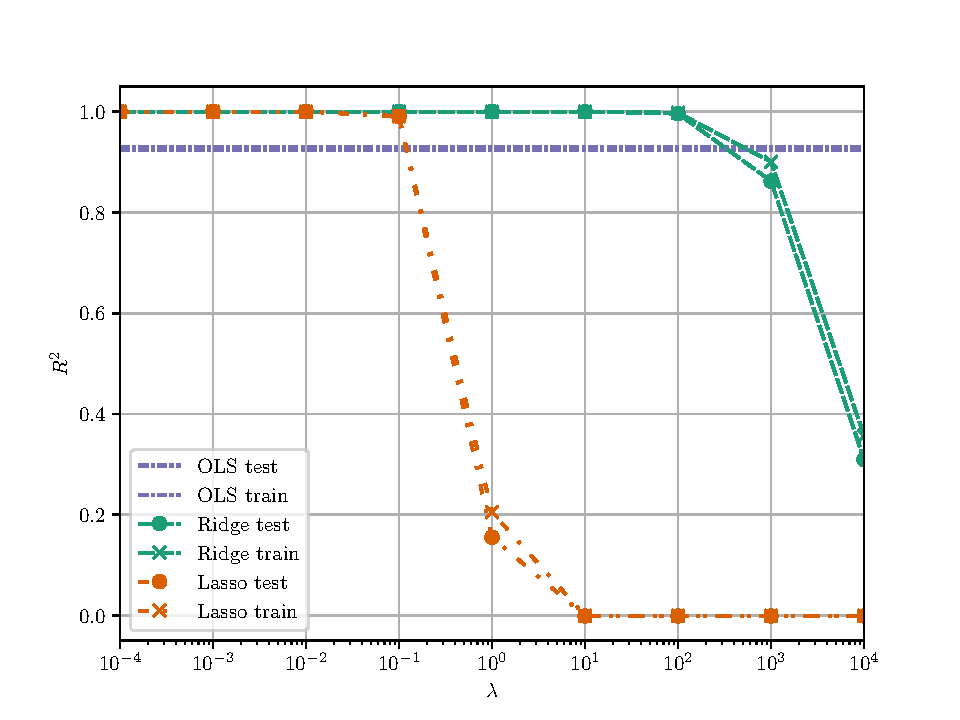
\includegraphics[scale=1.0]{../fig/r2_ols_ridge_lasso.pdf}
    \caption{$R^2$ score for different Ordinary Least Squares(OLS), Ridge and Lasso regression. Retrieved $N_\mathrm{train}=5000$ and $N_\mathrm{test}=5000$ on a 1D Ising model of size $L=20$.}
    \label{fig:linreg-r2}
\end{figure}

The bias-variance decomposition for Ridge and Lasso using bootstrap and cross validation can be viewed in figure \ref{fig:linreg-bias-variance-decomp-ridge} and \ref{fig:linreg-bias-variance-decomp-lasso}.

\begin{figure}[H]
    \centering
    \begin{subfigure}[b]{0.5\textwidth}
        \centering
        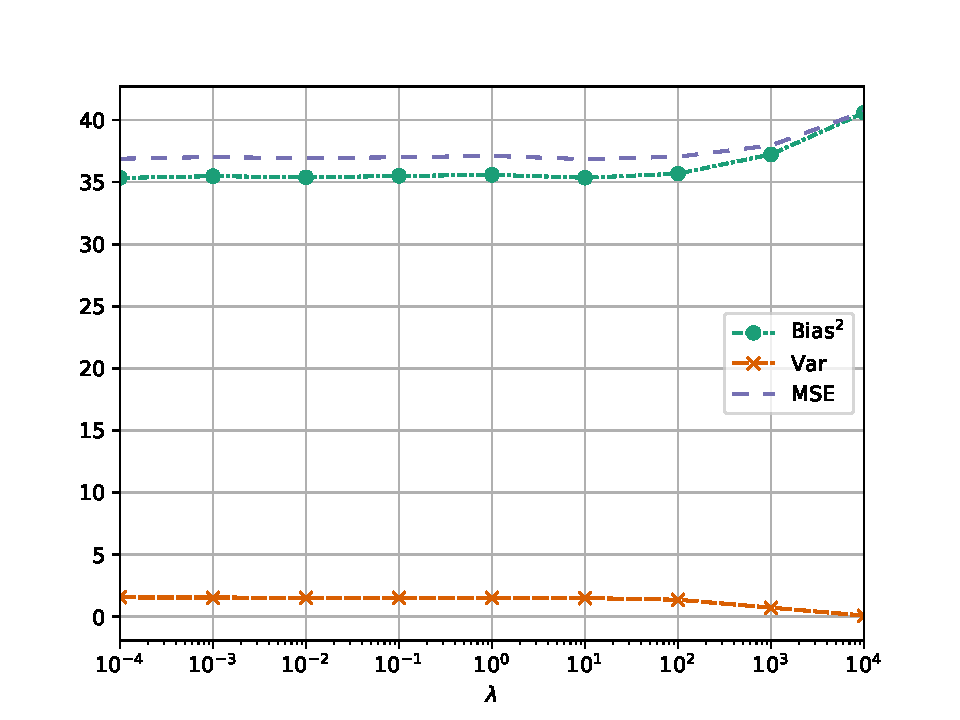
\includegraphics[scale=0.5]{../fig/ridge_bs_bias_variance_analysis.pdf}
        \caption{Bootstrap.}
        \label{fig:linreg-bias-variance-decomp-bs-ridge}
    \end{subfigure}%
    \begin{subfigure}[b]{0.5\textwidth}
        \centering
        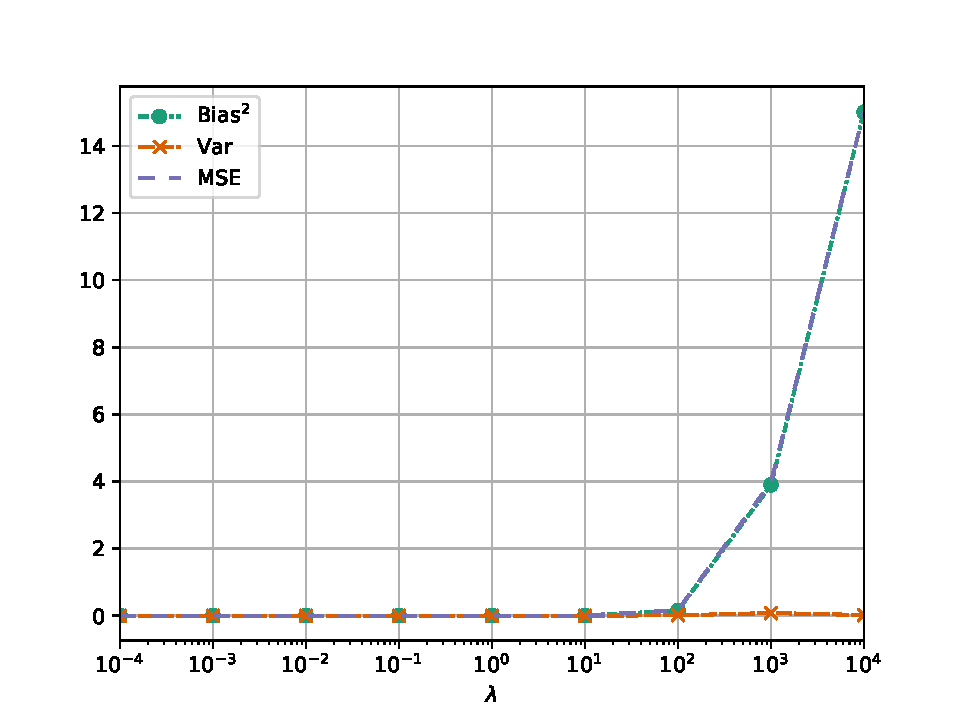
\includegraphics[scale=0.5]{../fig/ridge_cv_bias_variance_analysis.pdf}
        \caption{$k$-fold Cross Validation.}
        \label{fig:linreg-bias-variance-decomp-cv-ridge}
    \end{subfigure}
    \caption{A bias-variance decomposition of Ridge regression using bootstrapping\ref{fig:linreg-bias-variance-decomp-bs-ridge} and cross-validation\ref{fig:linreg-bias-variance-decomp-cv-ridge}.}
    \label{fig:linreg-bias-variance-decomp-ridge}
\end{figure}

\begin{figure}[H]
    \centering
    \begin{subfigure}[b]{0.5\textwidth}
        \centering
        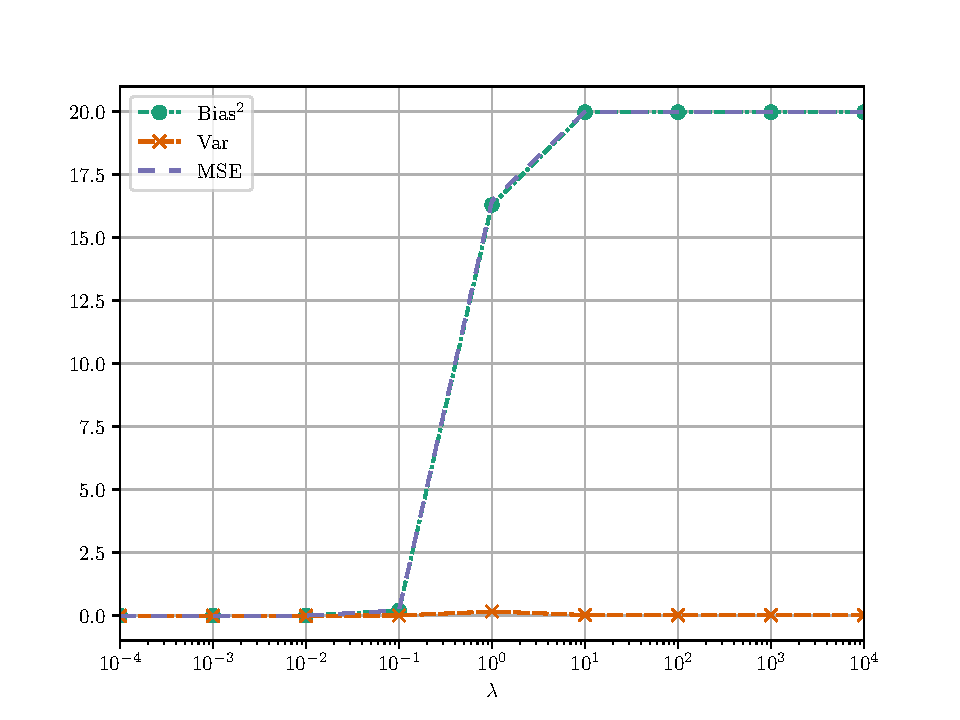
\includegraphics[scale=0.5]{../fig/lasso_bs_bias_variance_analysis.pdf}
        \caption{Bootstrap.}
        \label{fig:linreg-bias-variance-decomp-bs-lasso}
    \end{subfigure}%
    \begin{subfigure}[b]{0.5\textwidth}
        \centering
        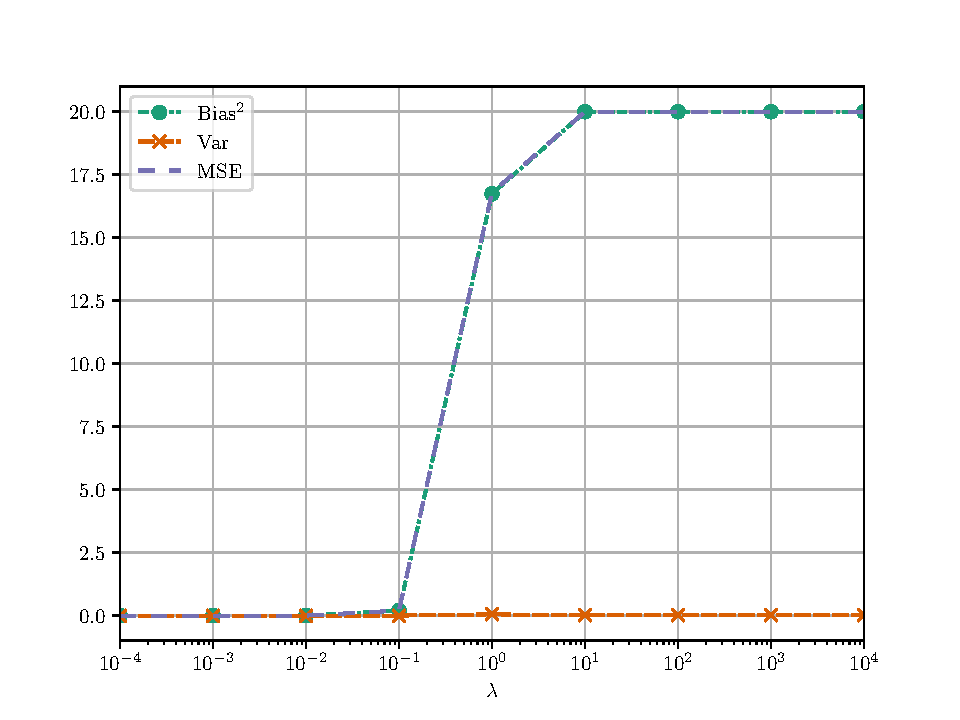
\includegraphics[scale=0.5]{../fig/lasso_cv_bias_variance_analysis.pdf}
        \caption{$k$-fold Cross Validation.}
        \label{fig:linreg-bias-variance-decomp-cv-lasso}
    \end{subfigure}
    \caption{A bias-variance decomposition of Lasso regression using bootstrapping\ref{fig:linreg-bias-variance-decomp-bs-lasso} and cross-validation\ref{fig:linreg-bias-variance-decomp-cv-lasso}.}
    \label{fig:linreg-bias-variance-decomp-lasso}
\end{figure}

\subsubsection{Fitting with a neural network}
By setting the output activation function to the identity and by having zero hidden layers, we are essentially performing a regression analysis on the 1D Ising model. We generate the same amount of data by inputing the same RNG(random number generator) seed. A fit using $N_\mathrm{train}=400$, $N_\mathrm{train}=5000$ and $N_\mathrm{test}=5000$ for $\lambda=10^{-3}, 10^{-1}, 10^1$ can be seen in figure \ref{fig:mlp_coefs}.

\begin{figure}[H]
    \centering
    \begin{subfigure}[b]{0.4\textwidth}
        \centering
        \includegraphics[trim={1.5cm 3.5cm 0 3.5cm},clip, scale=0.6]{../fig/{mlp_ising_1d_heatmap_lambda0.0001_N800}.pdf}
        \caption{$N_\mathrm{train}=400$, $\lambda=10^{-3}$}
        \label{fig:mlp-reg-heatmap400-lmb-3}
    \end{subfigure} \qquad \qquad \qquad
    \begin{subfigure}[b]{0.4\textwidth}
        \centering
        \includegraphics[trim={1.5cm 3.5cm 0 3.5cm},clip, scale=0.6]{../fig/{mlp_ising_1d_heatmap_lambda0.0001_N100000}.pdf}
        \caption{$N_\mathrm{train}=5000$, $\lambda=10^{-3}$}
        \label{fig:mlp-reg-heatmap5000-lmb-3}
    \end{subfigure} \\
        \begin{subfigure}[b]{0.4\textwidth}
        \centering
        \includegraphics[trim={1.5cm 3.5cm 0 3.5cm},clip, scale=0.6]{../fig/{mlp_ising_1d_heatmap_lambda0.1_N800}.pdf}
        \caption{$N_\mathrm{train}=400$, $\lambda=10^{-1}$}
        \label{fig:mlp-reg-heatmap400-lmb-1}
    \end{subfigure} \qquad \qquad \qquad
    \begin{subfigure}[b]{0.4\textwidth}
        \centering
        \includegraphics[trim={1.5cm 3.5cm 0 3.5cm},clip, scale=0.6]{../fig/{mlp_ising_1d_heatmap_lambda0.1_N100000}.pdf}
        \caption{$N_\mathrm{train}=5000$, $\lambda=10^{-1}$}
        \label{fig:mlp-reg-heatmap5000-lmb-1}
    \end{subfigure} \\
        \begin{subfigure}[b]{0.4\textwidth}
        \centering
        \includegraphics[trim={1.5cm 3.5cm 0 3.5cm},clip, scale=0.6]{../fig/{mlp_ising_1d_heatmap_lambda10.0_N800}.pdf}
        \caption{$N_\mathrm{train}=400$, $\lambda=10^1$}
        \label{fig:mlp-reg-heatmap400-lmb1}
    \end{subfigure} \qquad \qquad \qquad
    \begin{subfigure}[b]{0.4\textwidth}
        \centering
        \includegraphics[trim={1.5cm 3.5cm 0 3.5cm},clip, scale=0.6]{../fig/{mlp_ising_1d_heatmap_lambda10.0_N100000}.pdf}
        \caption{$N_\mathrm{train}=5000$, $\lambda=10^1$}
        \label{fig:mlp-reg-heatmap5000-lmb1}
    \end{subfigure} \\
    \caption{Heat map plot of the coefficients of $\bm{J}$ in \eqref{eq:1d-ising-linreg} using neural networks with different regularizations for $\lambda=10^{-3}, 10^{-1}, 10^1$.}
    \label{fig:mlp-coefs}
\end{figure}

The $R^2$ score of the neural network using L$^1$, L$^2$ and no regularization can be seen in figure \ref{fig:mlp-r2},
\begin{figure}[H]
    \centering
    \begin{subfigure}[b]{0.5\textwidth}
        \centering
        \includegraphics[scale=0.5]{../fig/{mlp_r2_ols_ridge_lasso800}.pdf}
        \caption{$N_\mathrm{train}=400$}
        \label{fig:mlp-r2-800}
    \end{subfigure}%
    \begin{subfigure}[b]{0.5\textwidth}
        \centering
        \includegraphics[scale=0.5]{../fig/{mlp_r2_ols_ridge_lasso100000}.pdf}
        \caption{$N_\mathrm{train}=5000$}
        \label{fig:mlp-r2-5000}
    \end{subfigure}
    \caption{$R^2$ score for the neural network using L$^1$ (Lasso), L$^2$ (Ridge) and no regularization (OLS). Retrieved $N_\mathrm{train}=400$ on the left and $N_\mathrm{train}=5000$ on the right, for a 1D Ising model of size $L=20$.}
    \label{fig:mlp-r2}
\end{figure}

% TODO: rerun mlp regression with N_samples = 10000 as I run for too much :|

\subsection{2D Ising model}
As stated in the section about the 2D Ising model \ref{sec:2d-ising-model}, the classification will focus on evaluating the phases of different lattice configurations, and wetter or not it is below or above a critical temperature. We begin by listing the results from the logistic regression.
\subsubsection{Classification through logistic regression}
In logistic regression we investigated the behavior of the classification and compared it to that of SciKit Learn\cite{scikit-learn}, using the standard logistic regression method\footnote{See \href{https://scikit-learn.org/stable/modules/generated/sklearn.linear_model.LogisticRegression.html}{Logistic Regression documentation}} and 
SciKit Learn's SGD(Stochastic Gradient Descent) implementation \footnote{See \href{https://scikit-learn.org/stable/modules/generated/sklearn.linear_model.SGDClassifier.html}{SGD documentation}}. This gave the results found in figure \ref{fig:logreg-accuracy-sklearn-comparison}.

\begin{figure}[H]
    \centering
    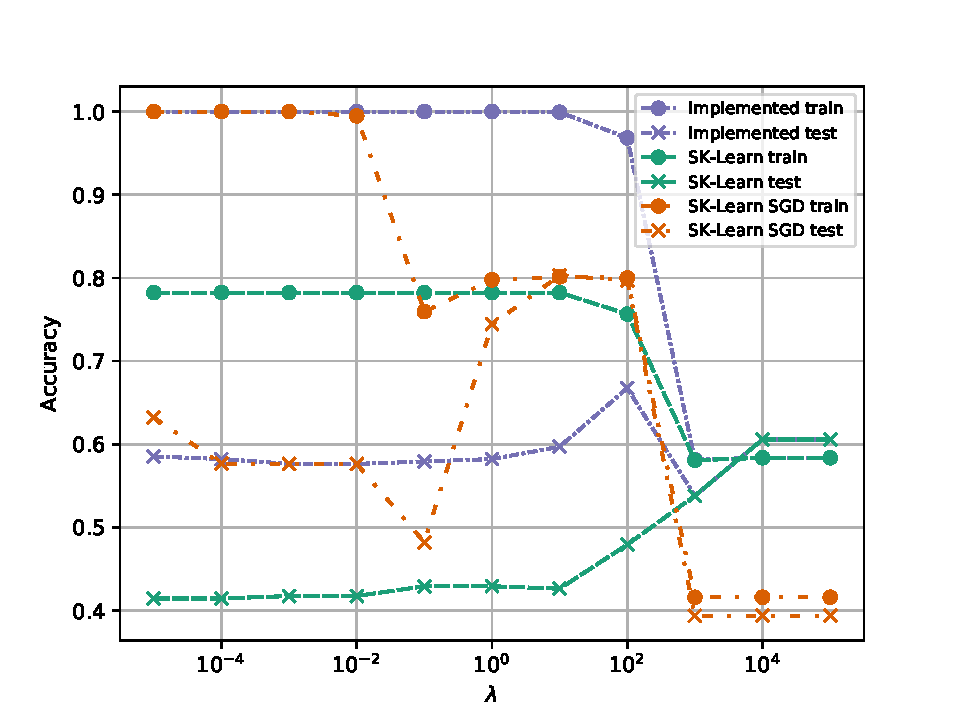
\includegraphics[scale=1.0]{../fig/logistic_accuracy_sklearn_comparison.pdf}
    \caption{The accuracy for our implementation of logistic regression versus that of SciKit learn.}
    \label{fig:logreg-accuracy-sklearn-comparison}
\end{figure}

\subsubsection{Classification through neural networks}
For classifying the states through a neural network, we looked at several different hyper parameters. All runs were made using $N_{samples}=10000$ except stated other wise. The training percent was 0.5. We start by comparing two different cost functions and their layer outputs,
\begin{itemize}
    \item Cross entropy with softmax layer output\eqref{eq:ce-mlp-cost}
    \item MSE with sigmoidal layer output.\eqref{eq:mse-mlp-cost}
\end{itemize}
These cost functions following behavior for epochs seen in following figure \ref{fig:mlp-cost-function-comparison},
\begin{figure}[H]
    \centering
    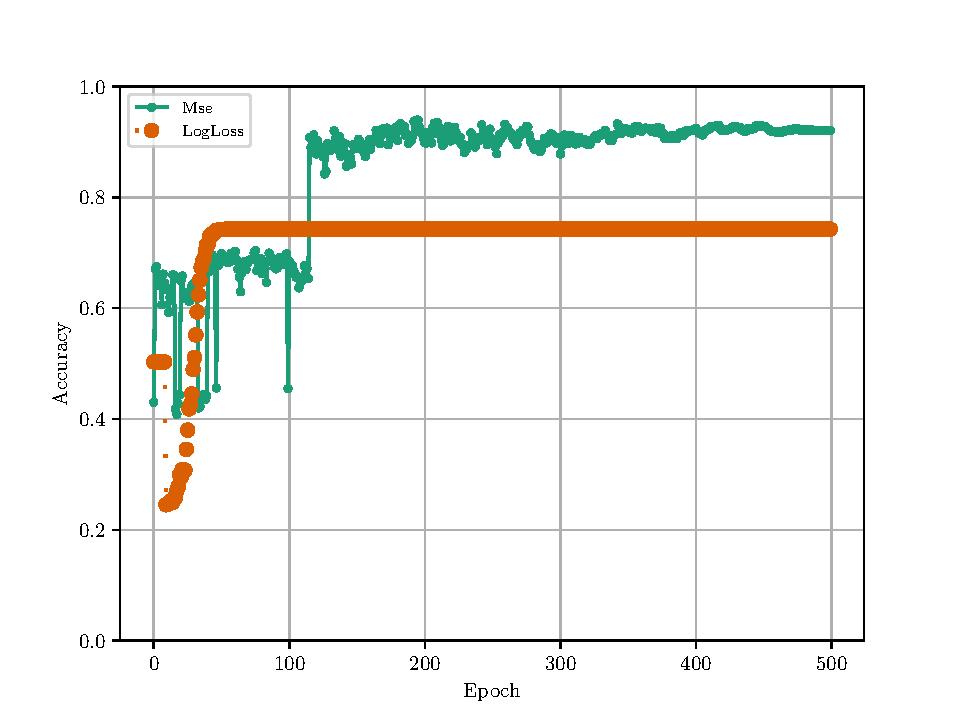
\includegraphics[scale=1.0]{../fig/mlp_epoch_cost_functions.pdf}
    \caption{A comparison in accuracy scores between the MSE and (CE) Cross Entropy loss functions over 500 epochs. The output layer for MSE is sigmoidal, the output layer for CE is softmax. The learning parameter was $\eta=0.001$ and we used the inverse learning rate\eqref{eq:inverse-eta}.}
    \label{fig:mlp-cost-function-comparison}
\end{figure}

We then wish to to investigate the effects of having different initial weights. Given the initial weights \textit{large} and \textit{default} as listed in section \ref{sec:nn-weights}, we get the results as seen in figure \ref{fig:mlp-epoch-init-weights},
\begin{figure}[H]
    \centering
    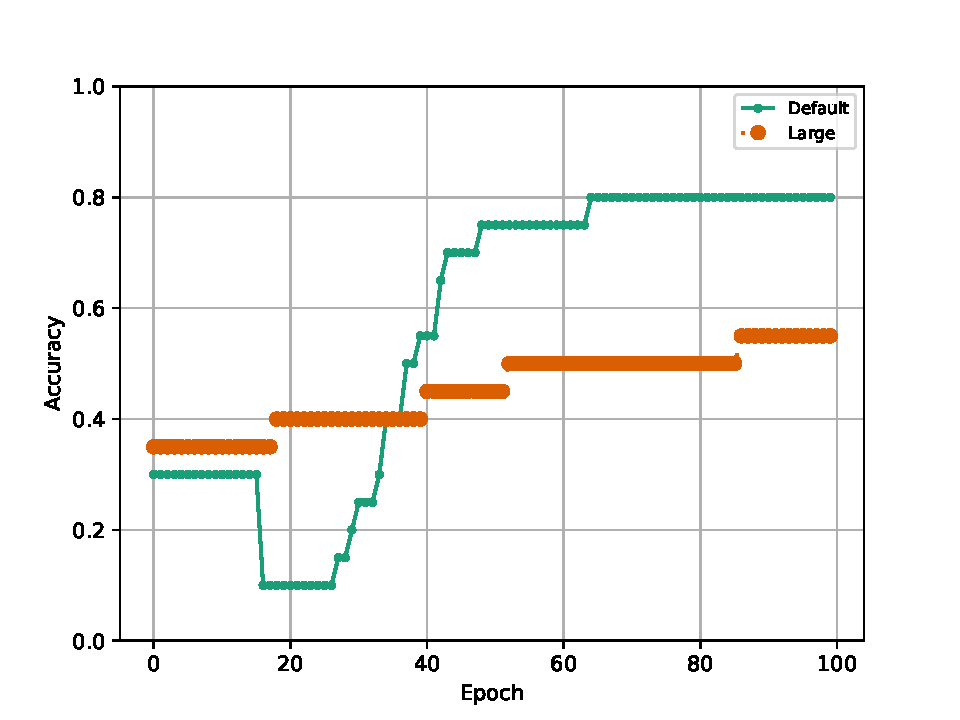
\includegraphics[scale=1.0]{../fig/mlp_epoch_weight_inits.pdf}
    \caption{A comparison in accuracy scores between the initial weights \textit{large} and \textit{default} as listed in section \ref{sec:nn-weights}. The run was for 500 epochs. The cost function was set to cross entropy and had softmax output activation. The learning parameter was $\eta=0.001$ and we used the inverse learning rate\eqref{eq:inverse-eta}.}
    \label{fig:mlp-epoch-init-weights}
\end{figure}

% skriv inn lambda ting her !=")#(097 21841 \\\\}Ʒ׶"

An investigation into different layer activations\ref{sec:layer-acts} was performed for both the MSE- and the CE-cost function. The results from MSE can be seen in figure 
\begin{figure}[H]
    \centering
    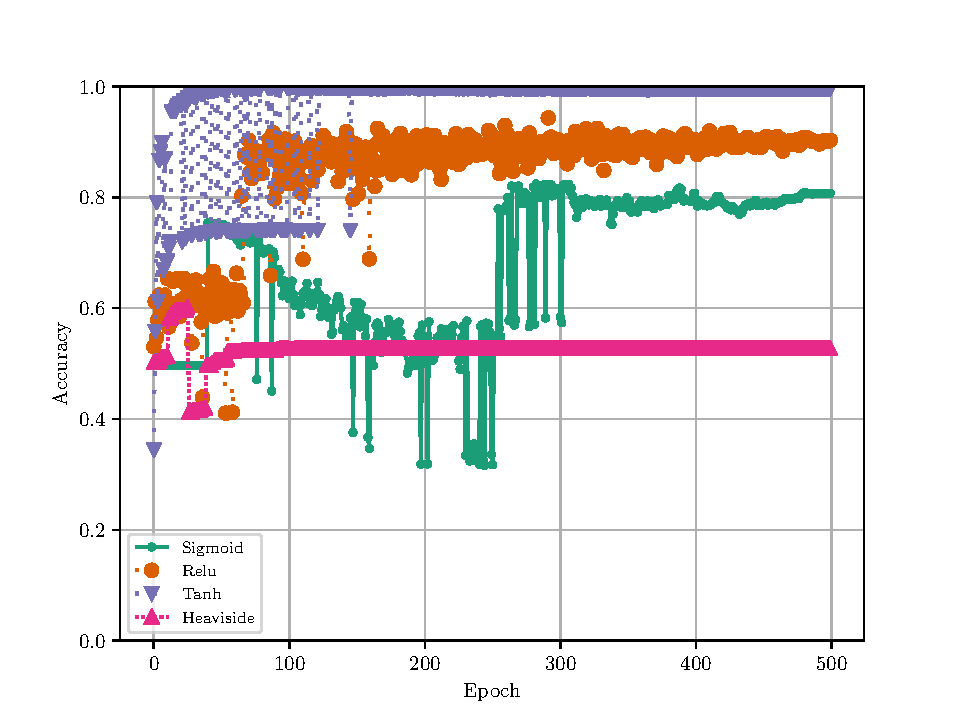
\includegraphics[scale=1.0]{../fig/mlp_epoch_activations_mse.pdf}
    \caption{A comparison in accuracy scores between the hidden layer activation functions(see section \ref{sec:layer-acts}) for MSE as cost function. The run was for 500 epochs. The learning rate was set with the inverse learning rate \eqref{eq:inverse-eta} with an $\eta_0=0.001$ and $\lambda=0.0$.}
    \label{fig:mlp-epoch-activations-mse}
\end{figure}
\begin{figure}[H]
    \centering
    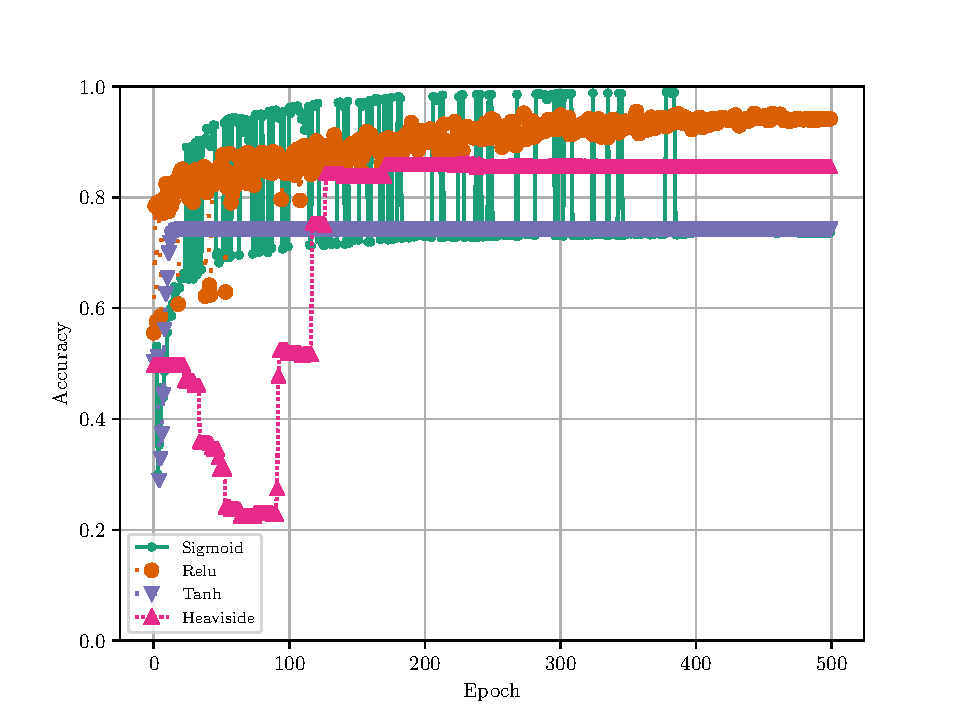
\includegraphics[scale=1.0]{../fig/mlp_epoch_activations_log_loss.pdf}
    \caption{A comparison in accuracy scores between the hidden layer activation functions(see section \ref{sec:layer-acts}) for cross entropy as cost function. The run was for 500 epochs. The learning rate was set with the inverse learning rate \eqref{eq:inverse-eta} with an $\eta_0=0.001$ and $\lambda=0.0$.}
    \label{fig:mlp-epoch-activations-log-loss}
\end{figure}

We then move on to an investigation for different L$^2$ regularization strengths $\lambda$ versus different constant learning rates $\eta$. A run with 500 epochs, cross entropy and sigmoidal hidden layer activation can be seen in figure \ref{fig:mlp-eta-lambda},
\begin{figure}[H]
    \centering
    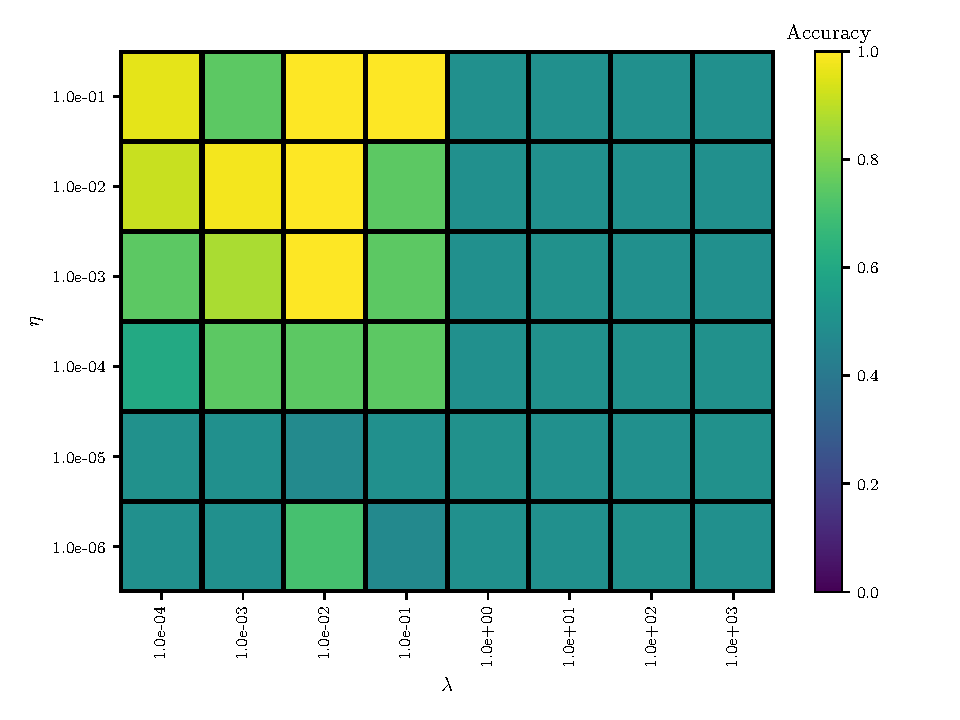
\includegraphics[scale=1.0]{../fig/mlp_lambda_eta.pdf}
    \caption{The accuracy as function of the L$^2$ regularization parameter $\lambda$ and constant training rate $\eta$. The run was for 500 epochs and with cross entropy as cost function, softmax output and sigmoidal hidden layer activation. The hidden layer was 10 neurons large.}
    \label{fig:mlp-eta-lambda}
\end{figure}

A comparison of the accuracy score\eqref{eq:mlp-accuracy} as a function of L$^2$ regularization parameter and hidden layer size(the neurons) can be viewed in figure \ref{fig:mlp-lambda-neurons}.
\begin{figure}[H]
    \centering
    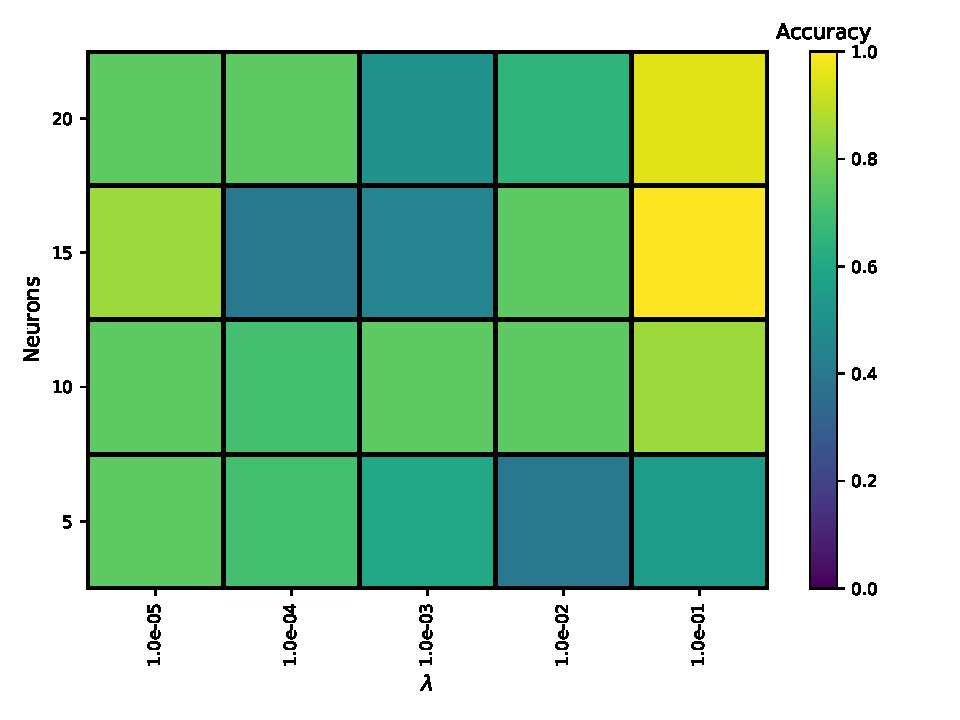
\includegraphics[scale=1.0]{../fig/mlp_lambda_neurons.pdf}
    \caption{The accuracy score as function of the L$^2$ regularization parameter $\lambda$ and the number of neurons. The run was for 500 epochs and with cross entropy as cost function, softmax output and sigmoidal hidden layer activation. The learning rate was set with the inverse learning rate \eqref{eq:inverse-eta} with an $\eta_0=0.001$.}
    \label{fig:mlp-lambda-neurons}
\end{figure}

The accuracy score\eqref{eq:mlp-accuracy} as a function of the hidden layer size(the neurons) and the training data size as percentage of of a $N_\mathrm{samples}=10000$ training data, can be viewed in figure \ref{fig:mlp-neurons-ts}.
\begin{figure}[H]
    \centering
    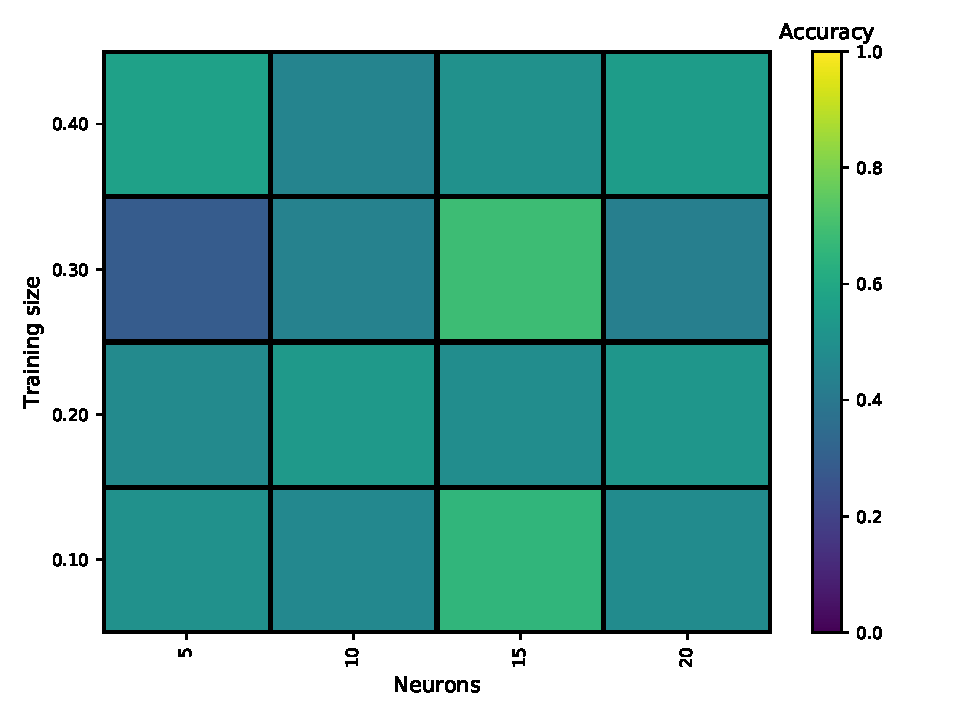
\includegraphics[scale=1.0]{../fig/mlp_neurons_training_size.pdf}
    \caption{The accuracy score as function of the number of neurons and the training data size percentage of $N_\mathrm{samples}=10000$. The run was for 500 epochs and with cross entropy as cost function, softmax output and sigmoidal hidden layer activation. The learning rate was set with the inverse learning rate \eqref{eq:inverse-eta} with an $\eta_0=0.001$ and $\lambda=0.0$. }
    \label{fig:mlp-neurons-ts}
\end{figure}

The accuracy score\eqref{eq:mlp-accuracy} as a function of the hidden layer size(the neurons) and the learning rate $\eta$, can be viewed in figure \ref{fig:mlp-neurons-ts}.
\begin{figure}[H]
    \centering
    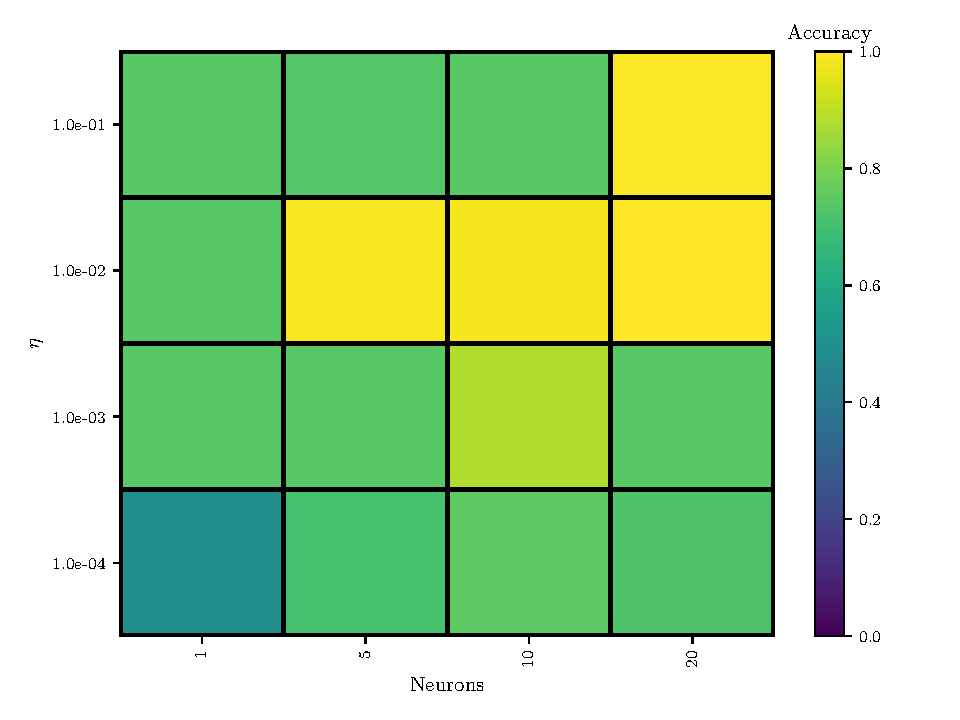
\includegraphics[scale=1.0]{../fig/mlp_neurons_eta.pdf}
    \caption{The accuracy score as function of the number of neurons and the learning rate $\eta$. The run was for 500 epochs and with cross entropy as cost function, softmax output and sigmoidal hidden layer activation. The regularization strength was set to $\lambda=0.0$}.
    \label{fig:mlp-neurons-eta}
\end{figure}

The accuracy score\eqref{eq:mlp-accuracy} as a function of L$^2$ regularization strength $\lambda$ and the mini batch size in the SGD\ref{alg:sgd}, can be viewed in figure \ref{fig:mlp-lambda-mb}.
\begin{figure}[H]
    \centering
    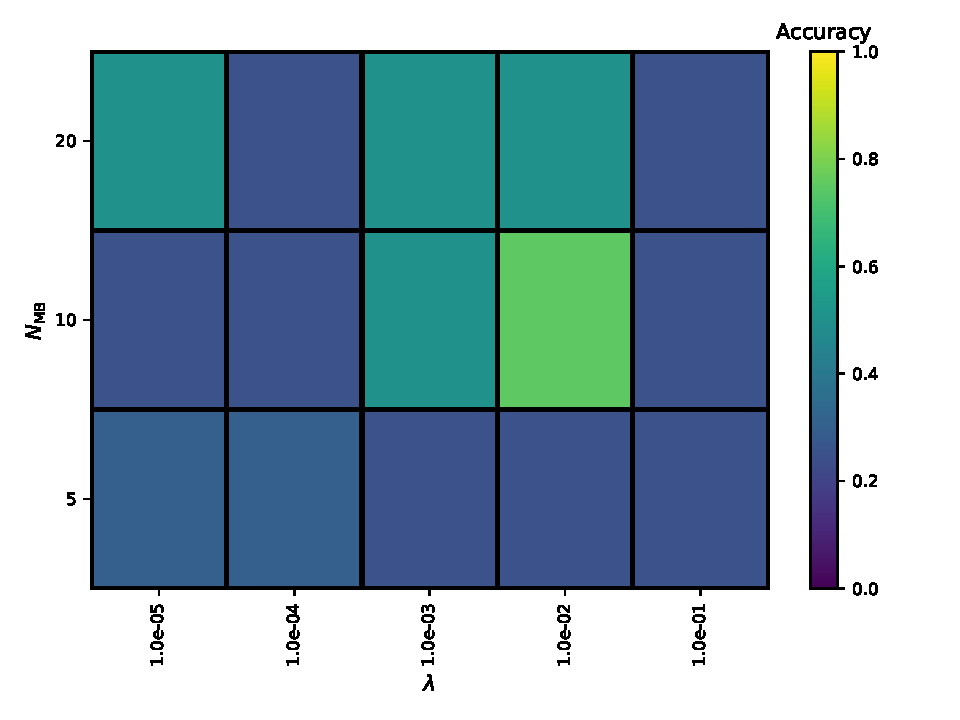
\includegraphics[scale=1.0]{../fig/mlp_lambda_mini_batch_size.pdf}
    \caption{The accuracy score as function of the  L$^2$ regularization strength $\lambda$ and the mini batch size in the SGD\ref{alg:sgd}. The run was for 500 epochs and with cross entropy as cost function, softmax output and sigmoidal hidden layer activation and the inverse learning rate \eqref{eq:inverse-eta} with $\eta_0=0.001$.}
    \label{fig:mlp-lambda-mb}
\end{figure}

After choosing following optimal parameters, we get 
\begin{table}[H]
    \centering
    \begin{tabular}{l l} % 6 columns
        \specialrule{.1em}{.05em}{.05em}
        $N_\mathrm{neurons}$    & 10 \\
        $\lambda$               & 0.1 \\
        $N_\mathrm{mb}$         & 20 \\
        $N_\mathrm{epochs}$     & 500 \\
        $\eta$ (constant)       & 0.001 \\
        \specialrule{.1em}{.05em}{.05em}
    \end{tabular}
    \caption{Based on the different fitting procedures, these fit parameters were determined to be the best. The polynomial fitted was of degree $6$.}
    \label{tab:opt_ols_result}
\end{table}

\begin{figure}[H]
    \centering
    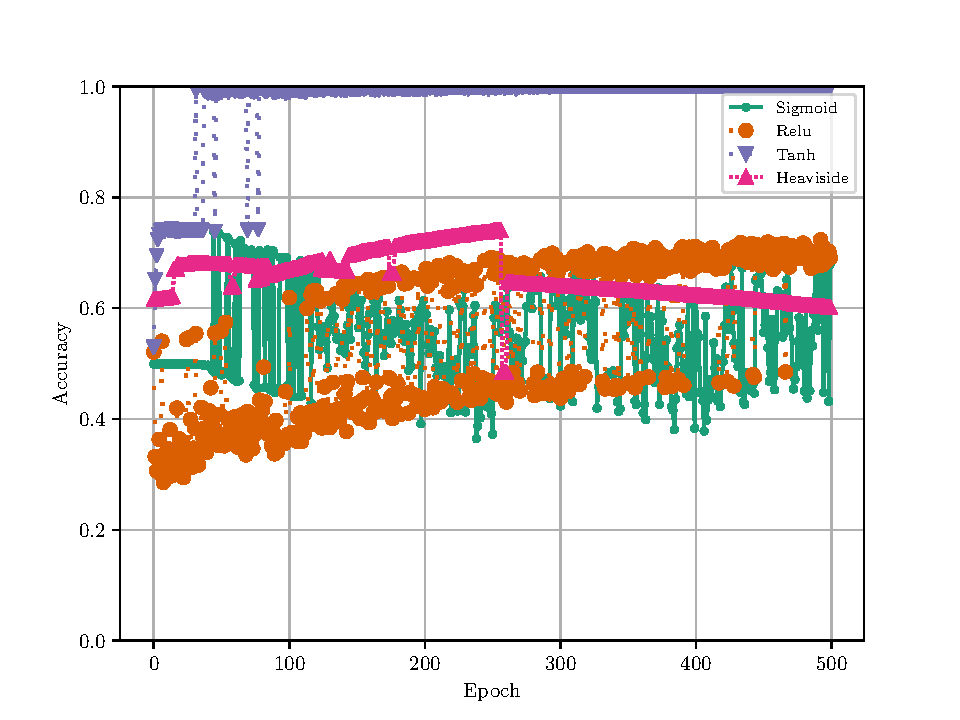
\includegraphics[scale=1.0]{../fig/mlp_epoch_activations_mse2.pdf}
    \caption{A comparison in accuracy scores between the hidden layer activation functions(see section \ref{sec:layer-acts}) for MSE as cost function using \textit{optimal parameters}. The optimal parameters can be viewed in table .}
    \label{fig:mlp-epoch-activations-mse-optimal}
\end{figure}

\begin{figure}[H]
    \centering
    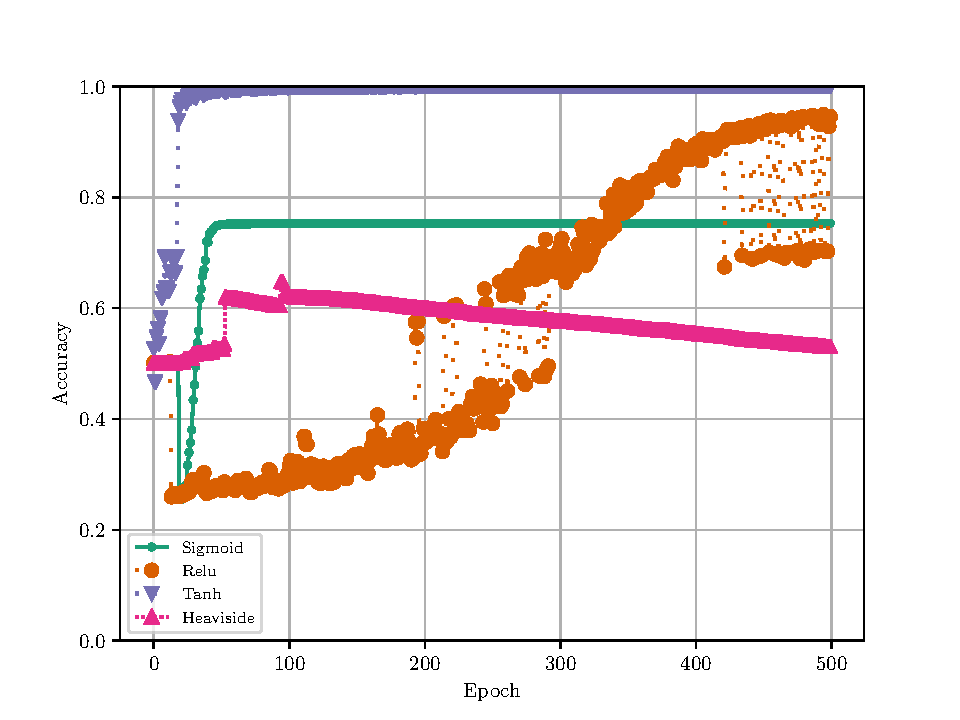
\includegraphics[scale=1.0]{../fig/mlp_epoch_activations_log_loss2.pdf}
    \caption{A comparison in accuracy scores between the hidden layer activation functions(see section \ref{sec:layer-acts}) for cross entropy as cost function using \textit{optimal parameters}. The optimal parameters can be viewed in table.}
    \label{fig:mlp-epoch-activations-log-loss-optimal}
\end{figure}

%%%%%%%%%%%%%%%%%%%%%%%%%%%%%%%%
\section{Discussion}
% <<<<<<< HEAD

\subsection{1D Ising model}
\subsubsection{Fitting with linear regression}
By examining the results from figure \ref{fig:bias-var-franke} illustrates the effect of different $\lambda$-values. The diagonal line illustrates the particle we are looking at and the pixels to its immediate left and right are the nearest neighbours. It is clear from this figure that even though we assumed that all particles interact with each other, only the neighbouring particles will have a profound effect on each other. For Lasso, it seems that the optimal $\lambda$ is either $10^{-3}$ or $10^{-1}$. This is agreeable with the results of Metha et al \cite{2018arXiv180308823M} who found $10^{-2}$ to be the optimal parameter. For Ridge and OLS we can not seem to see any big difference between the different $\lambda$'s. The inability to find the best $\lambda$ for OLS and Ridge and the fact that we do not have a clear optimal parameter for Lasso indicates that we should have gathered more data. 

However, by looking at figure \ref{fig:linreg-r2} we can see that there is little change in the R2-score for different $\lambda$-values, indicating that it would not matter if we generated many more plots. They would most likely stay the same. It is also clear that Lasso is the most sensitive of the models, loosing ground to the other regression methods already at $\lambda = 10^{-1}$. The R2-score for Ridge starts to decline at about $\lambda = 10^{3}$, while OLS seems to maintain its quality over all $\lambda$'s. 

This trend is further confirmed by figure \ref{fig:fig:linreg-bias-variance-decomp-ridge} and \ref{fig:linreg-bias-variance-decomp-lasso} where we have used Bootstrap and $k$-fold validation to verify our results. As we can see, the variance stays about the same for all $\lambda$-values, but MSE and therefore, the bias increases. This shift in bias also happens around $\lambda = 10^{-1}$ for Lasso and $\lambda = 10^{3}$ for Ridge as the R2-score did as well.

\subsubsection{Fitting with a neural network}
Repeating the calculations using a neural net with zero hidden layers and the identity function as the activation function gives us the opportunity to repeat the above calculations using a neural net instead. As we can see from figure \ref{fig:mlp-coefs}, the difference in $N_{\text{train}}$ had little effect, but the change in $\lambda$ was significant. The change between OLS, Ridge and Lasso also represent a change in regularisation from no regularisation to L$^2$ to L$^1$ respectively. 

In contrast to the linear regression case, there is a difference between $\lambda = 10^{-3}$ and $\lambda = 10^{-1}$. The diagonal lines once removed which signifies the nearest neighbours are about as strong for both parameters, however, there is a noticeable decrease in noise for the $\lambda = 10^{-1}$ case. Furthermore, we must note that the use of the parameter $\lambda = 10^{1}$ is more devastating for Ridge than Lasso this time around. Lasso looses a lot of information, but for Ridge the significant of nearest neighbours disappears completely. The same trend is once again evident for the R2-score plotted in figure \ref{fig:mlp-r2}. However, with this representation we can see that increasing $N_{\text{train}}$ decreases the difference between the test and train data. This is as expected.

The difference between \ref{fig:mlp-coefs} and \ref{fig:reg-coef-heatmap} is due to the way SciKit-Learn optimizes the Lasso function. Since we are utlizing SciKit-Learn in our Lasso regression, the way it uses coordinate descent as its optimization method, it only finds one part of the diagonal.

\subsection{2D Ising model}
\subsubsection{Classification through logistic regression}
From figure \ref{fig:logreg-accuracy-sklearn-comparison} we can compare the accuracy of our implemented logistic regression method to that of SKLearn. Furthermore, we can compare our results to those of Metha et al. \cite{2018arXiv180308823M}. What is peculiar in our case is that SKlearn with Stochastic Gradient Descent (SGD) is very varied over the different $\lambda$-values, while Metha et al. have quite stable values. Both standard SKlearn and the implemented methods have stable accuracies, with the implemented train being the clear winner. A reason for this unexpected variation in accuracy for SGD might be that we perform the analyses on less data than those of Metha et al. causing our SGD to jump more randomly back and forth for higher $\lambda$-values. If the experiment was to be repeated we would double check that the SKlearn with SGD was correctly used and give it more data. Our implemented data have performed better than those of Metha et al., which is positive. However, this might also indicate that we have implemented something wrong and are just lucky. If this experiment were to be repeated we would also double check our implementation and run it over more data to truly test if we are just lucky or if our method is actually better.

\subsubsection{Classification through neural networks}
To find the optimal solution using the neural net we implemented many different features to our Neural Net (NN). All these results can be viewed in figures \ref{fig:mlp-cost-function-comparison} - \ref{fig:mlp-epoch-activations-log-loss}. We then moved on to trying to find the optimal parameters in figures \ref{fig:mlp-eta-lambda} - \ref{fig:mlp-lambda-mb}. 

Our initial results in figure \ref{fig:mlp-cost-function-comparison} gives us a comparison of using either MSE or LogLoss as a cost function. The latter cost function ca nthen be directly compared to our logistic regression results in figure \ref{fig:logreg-accuracy-sklearn-comparison}. As we can see, the LogLoss accuracy increases significantly over the first 20-30 epochs before varying until we reach some more than 300 epochs. After this the accuracy is almost 1.0 which seems a bit to good to be true. The MSE stays at around 0.75, which is quite comparable to the results of the logistic regression above. 

Comparing the initial weights between the default and large as in figure \ref{fig:mlp-epoch-init-weights}, we see a similar trend. For smaller number of epochs, the accuracy increases quite drastically until it becomes stable a bit before the 100 epochs mark. Once the stable accuracy is reached, the Large initial weights perform best, however, there is not that big of a difference. These results are also comparable to the logistic regression above and seem to be a bit worse than the implemented train, but better than the implemented test. 

Furthermore, figures \ref{fig:mlp-epoch-activations-mse} and \ref{fig:mlp-epoch-activations-log-loss} indicates that changing the activation function will have an effect on the accuracy as well. This is to be expected. The Heaviside function was added for historical reasons and even though it is the loser when both cost functions are considered, it is clear why this function was the initial function which was used at the advent of Neural Nets and made scientists want more. In our modern times the other functions are more used and Relu is the clear accuracy winner for MSE and the Sigmoid and Relu are so close that they are almost indistinguishable for cross entropy. This indicates that Relu should be the optimal activation function, regardless of cost function. 

No Neural Net is only made up of the activation and cost function, we also need to do an in-depth analyses of the different variables. From figure \ref{fig:mlp-eta-lambda} it seems as though a smaller $\lambda$ and larger is $\eta$ is generally better until we reach a limit. From this figure it seems as though a learning rate of $\eta = 1.0e-02$ and $\lambda = 1.0e-02$ gives us the optimal accuracy. 
 
However, there are more concerns to take into account. Figure \ref{fig:mlp-lambda-neurons} seems to point towards a decrease in $\lambda$ and an increase in neurons is almost always better. It is also clear that even though it seems to increase, it also seems to reach a plateau where further increases in neurons and decreases in $\lambda$ may have an effect. As this will also increase computational time, it seems as though $\lambda = 1.0e-02$ and 30 neurons gives us the optimal balance between high accuracy and decreased computational time. 

Similarly, figure \ref{fig:mlp-neurons-ts} can be interpreted as training sets around 0.5 and large number of neurons gives us the optimal accuracy. It also seems as though the number of neurons is the most significant parameter of these two as all neuron columns seem to have quite similar accuracy, independent of training size, compared to the difference in accuracy of the training size rows. In this case it seems as though a training size of 0.5 with 20 or 30 neurons would be optimal. 
% =======
% >>>>>>> 444cc744f406ad703fe2c81cac764dbd083e7e71

Given the changes in learning rate compared to number of neurons displayed in figure \ref{fig:mlp-neurons-eta}, we see similar tendencies. An increase in neurons and an increase in learning rate is positive. However, the effect of increasing learning rate decreases once we pass $\eta = 1.0e-02$. The optimal learning rate is therefore $\eta = 1.0e-02$, but the accuracy seems to be quite similar for number of neurons from five and above. 
 
Finally, \ref{fig:mlp-lambda-mb} gives us quite unambiguous results. As $\lambda = 1.0e-02$ has been dominating the previous results, it is tempting to see the same here as well. And there are indications that a batch size of 30 and $\lambda = 1.0e-02$ are the optimal values, however, there are no trends significant enough to say this with certainty. 

Figures \ref{fig:mlp-epoch-activations-mse-optimal} - \ref{fig:mlp-epoch-activations-log-loss-optimal} is a repeat of figures \ref{fig:mlp-cost-function-comparison} and \ref{fig:mlp-epoch-activations-log-loss} with optimal settings. We can see that with the optimal settings, $\tanh$ is the superior activation function. This indicates that neural nets with $\tanh$ as activation function will most likely be the optimal method for solving the classification problems presented in this experiment.
\subsection{Future works}

For future works it would be desirable to look further into why our logistic implementation outperforms those of SKlearn and why the SGD method varies as it does. It would also be preferable to find better results for how many mini batches would be optimal for Neural Nets. One can also do better analyses by increasing the amount of data, but this is also left to the future and future, more powerful computers.

% <<<<<<< HEAD
% =======
% The difference in \ref{fig:mlp-coefs} and in \ref{fig:reg-coef-heatmap} is due to the way SciKit-Learn optimizes the Lasso function. Since we are utlizing SciKit-Learn in our Lasso regression, the way it uses coordinate descent as its optimization method, it only finds one part of the diagonal.
% \subsection{2D Ising model}
% \subsubsection{Classification through logistic regression}
% From figure \ref{fig:logreg-accuracy-sklearn-comparison} we can compare the accuracy of our implemented logistic regression method to that of SKLearn. Furthermore, we can compare our results to those of Metha et al. \cite{2018arXiv180308823M}. What is peculiar in our case is that SKlearn with Stochastic Gradient Descent (SGD) is very varied over the different $\lambda$-values, while Metha et al. have quite stable values. Both standard SKlearn and the implemented methods have stable accuracies, with the implemented train being the clear winner. A reason for this unexpected variation in accuracy for SGD might be that we perform the analyses on less data than those of Metha et al. causing our SGD to jump more randomly back and forth for higher $\lambda$-values. If the experiment was to be repeated we would double check that the SKlearn with SGD was correctly used and give it more data. Our implemented data have performed better than those of Metha et al., which is positive. However, this might also indicate that we have implemented something wrong and are just lucky. If this experiment were to be repeated we would also double check our implementation and run it over more data to truly test if we are just lucky or if our method is actually better.
% \subsubsection{Classification through neural networks}
% To find the optimal solution using the neural net we implemented many different features to our Neural Net (NN). All these results can be viewed in figures \ref{fig:mlp-cost-function-comparison} - \ref{fig:mlp-epoch-activations-log-loss}. We then moved on to trying to find the optimal parameters in figures \ref{fig:mlp-eta-lambda} - \ref{fig:mlp-lambda-mb}. \\ \\
% Our initial results in figure \ref{fig:mlp-cost-function-comparison} gives us a comparison of using either MSE or LogLoss as a cost function. The latter cost function ca nthen be directly compared to our logistic regression results in figure \ref{fig:logreg-accuracy-sklearn-comparison}. As we can see, the LogLoss accuracy increases significantly over the first 20-30 epochs before varying until we reach some more than 300 epochs. After this the accuracy is almost 1.0 which seems a bit to good to be true. The MSE stays at around 0.75, which is quite comparable to the results of the logistic regression above. \\
% Comparing the initial weights between the default and large as in figure \ref{fig:mlp-epoch-init-weights}, we see a similar trend. For smaller number of epochs, the accuracy increases quite drastically until it becomes stable a bit before the 100 epochs mark. Once the stable accuracy is reached, the Large initial weights perform best, however, there is not that big of a difference. These results are also comparable to the logistic regression above and seem to be a bit worse than the implemented train, but better than the implemented test. \\ \\
% Furthermore, figures \ref{fig:mlp-epoch-activations-mse} and \ref{fig:mlp-epoch-activations-log-loss} indicates that changing the activation function will have an effect on the accuracy as well. This is to be expected. The Heaviside function was added for historical reasons and even though it is the loser when both cost functions are considered, it is clear why this function was the initial function which was used at the advent of Neural Nets and made scientists want more. In our modern times the other functions are more used and Relu is the clear accuracy winner for MSE and the Sigmoid and Relu are so close that they are almost indistinguishable for cross entropy. This indicates that Relu should be the optimal activation function, regardless of cost function. \\
% No Neural Net is only made up of the activation and cost function, we also need to do an in-depth analyses of the different variables. From figure \ref{fig:mlp-eta-lambda} it seems as though a smaller $\lambda$ and larger is $\eta$ is generally better until we reach a limit. From this figure it seems as though a learning rate of $\eta = 1.0e-02$ and $\lambda = 1.0e-02$ gives us the optimal accuracy. \\ 
% However, there are more concerns to take into account. Figure \ref{fig:mlp-lambda-neurons} seems to point towards a decrease in $\lambda$ and an increase in neurons is almost always better. It is also clear that even though it seems to increase, it also seems to reach a plateau where further increases in neurons and decreases in $\lambda$ may have an effect. As this will also increase computational time, it seems as though $\lambda = 1.0e-02$ and 30 neurons gives us the optimal balance between high accuracy and decreased computational time. \\
% Similarly, figure \ref{fig:mlp-neurons-ts} can be interpreted as training sets around 0.5 and large number of neurons gives us the optimal accuracy. It also seems as though the number of neurons is the most significant parameter of these two as all neuron columns seem to have quite similar accuracy, independent of training size, compared to the difference in accuracy of the training size rows. In this case it seems as though a training size of 0.5 with 20 or 30 neurons would be optimal. \\
% Given the changes in learning rate compared to number of neurons displayed in figure \ref{fig:mlp-neurons-eta}, we see similar tendencies. An increase in neurons and an increase in learning rate is positive. However, the effect of increasing learning rate decreases once we pass $\eta = 1.0e-02$. The optimal learning rate is therefore $\eta = 1.0e-02$, but the accuracy seems to be quite similar for number of neurons from five and above. \\ 
% Finally, \ref{fig:mlp-lambda-mb} gives us quite unambiguous results. As $\lambda = 1.0e-02$ has been dominating the previous results, it is tempting to see the same here as well. And there are indications that a batch size of 30 and $\lambda = 1.0e-02$ are the optimal values, however, there are no trends significant enough to say this with certainty. \\ \\
% Figures \ref{fig:mlp-epoch-activations-mse-optimal} - \ref{fig:mlp-epoch-activations-log-loss-optimal} is a repeat of figures \ref{fig:mlp-cost-function-comparison} and \ref{fig:mlp-epoch-activations-log-loss} with optimal settings. We can see that with the optimal settings, $\tanh$ is the superior activation function. This indicates that neural nets with $\tanh$ as activation function will most likely be the optimal method for solving the classification problems presented in this experiment.
% >>>>>>> 444cc744f406ad703fe2c81cac764dbd083e7e71
% \subsection{Future works}
% For future works it would be desirable to look further into why our logistic implementation outperforms those of SKlearn and why the SGD method varies as it does. It would also be preferable to find better results for how many mini batches would be optimal for Neural Nets. One can also do better analyses by increasing the amount of data, but this is also left to the future and future, more powerful computers.


%%%%%%%%%%%%%%%%%%%%%%%%%%%%%%%%
\documentclass[11pt]{article}

\usepackage[utf8]{inputenc}
\usepackage{mathtools}
\usepackage{amsmath}
\usepackage{amsfonts}
\usepackage{enumerate}

% For proper referencing in article
\usepackage{hyperref}
\usepackage{url}

% For figures and graphics'n stuff
\usepackage{graphicx}
\usepackage{caption}
\usepackage{subcaption}
% \usepackage{tabularx}
\usepackage{float}

% For proper appendices
\usepackage[toc,page]{appendix}

% Algorithm packages
\usepackage{algorithm}
\usepackage{algorithmicx}
\usepackage{algpseudocode}

% For bold math symbols
\usepackage{bm}
\usepackage{xcolor}

% For customized hlines in tables
\usepackage{ctable}

% For having latex symbols in section titles
\usepackage{epstopdf}

% For proper citations
% \usepackage[round, authoryear]{natbib}
\usepackage[numbers]{natbib} 

% For fixing large table height
\usepackage{a4wide}

% Remembrance and checking
\newcommand{\husk}[1]{\color{red} #1 \color{black}}
\newcommand{\sjekk}[1]{\color{violet} #1 \color{black}}

\DeclareMathOperator{\sign}{sign}
\DeclareMathOperator*{\argmin}{argmin}
\DeclareMathOperator*{\CO}{\mathcal{C}}


% \title{FYS-STK4155: Project 2}
\title{Exploring the hyperspace of Machine Learning parameters}
\author{Eirik Ramsli Hauge, Joakim Kalsnes, Hans Mathias Mamen Vege}
\date{\today}

\begin{document}
\section{Conclusion}
We found that although both linear and logistic regression can be used, neural nets that are correctly tuned will give better scores. From our experiment, this is evident from the increase in R2 and accuracy score when comparing linear and logistic regression to their neural net counterparts respectively. For our linear regression, we found similar results to previous experiments and our results for logistic regression were different from those of Metha et al.. The reason for this difference is left to future experiments to decipher, but as it stands now, the implemented logistic regression was the superior method. For our neural net, the optimal parameters were a learning rate of $\eta = 1.0e-02$, $\lambda = 1.0e-02$, 20 neurons, 500 epochs and a mini batch size of 30. It was also evident that a neural net with $\tanh$ as activation function was the optimal neural net in our case.
\end{document}

%%%%%%%%%%%%%%%%%%%%%%%%%%%%%%%%
Put stuff like Bootstrapping, kfold CV, OLS/Ridge/Lasso regression here.

\subsection{A refresher on linear regression}
% Move this to appendix!
\subsubsection{Ridge regression}
\subsubsection{Lasso regression}

\subsection{Bootstrapping}
\subsection{k-fold Cross-Validation}


%%%%%%%%%%%%%%%%%%%%%%%%%%%%%%%%
\bibliographystyle{plainnat}
\bibliography{bibliography/lib.bib}


\end{document}
